% !TEX root = /media/ueslei/Ueslei/INPE/PCI/Projetos/Guia_COAWST/main.tex
\chapterimage{header.jpg}
\chapter{Construindo os pesos entre grades com o SCRIP}
\bigskip
\section{Construindo os pesos}
\bigskip
\noindent Como visto na seção \textcolor{bleu_cite}{\ref{scripsecao}}, o SCRIP é empregado para interpolar os pesos entre duas ou mais grades de modelos diferentes. No COAWST, o pacote foi modificado para gerar somente um arquivo NetCDF que sera utilizado durante as integrações.
\bigskip

\noindent O diretório do SCRIP está localizado em:
\bigskip

\begin{bashcode}
/home/nome.sobrenome/COAWST/Lib/SCRIP
\end{bashcode}
\bigskip

\noindent Dentro da pasta, procure pelo arquivo com extensão \textit{.in}. Como no exemplo da Figura \textcolor{bleu_cite}{\ref{scripinnedit}}:

\begin{figure}[H]
    \centering
    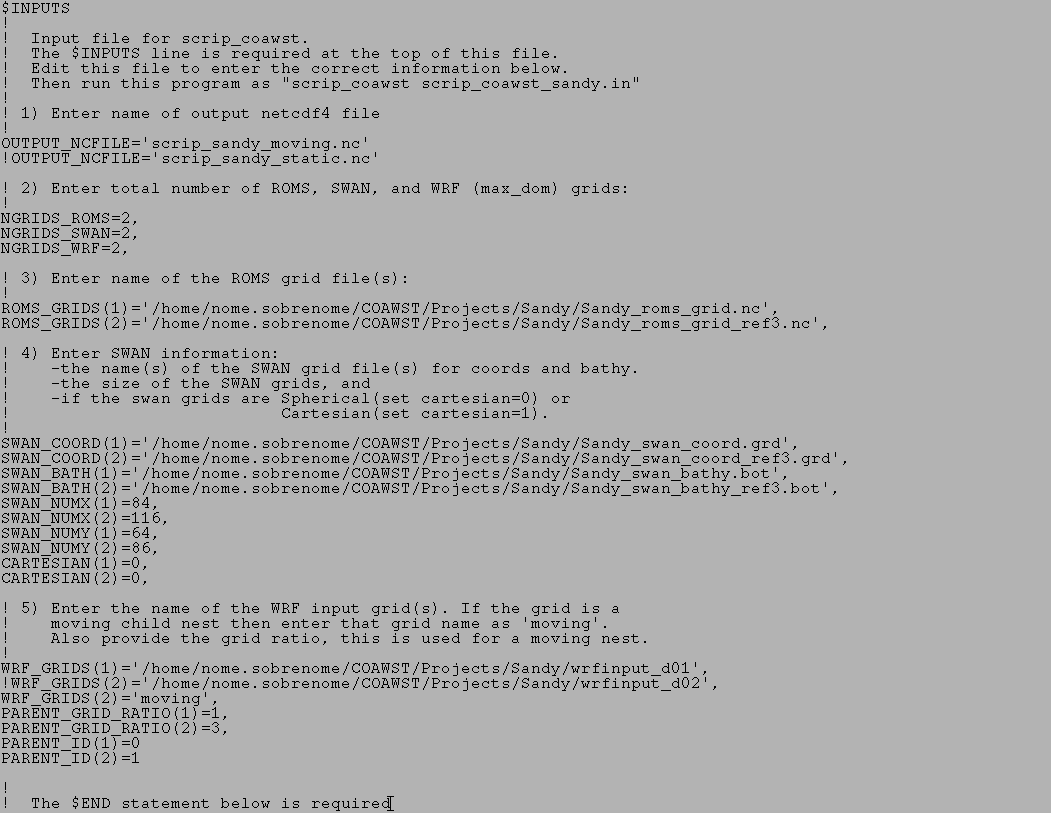
\includegraphics[width=0.65\textwidth]{scripin.png}
    \caption{Arquivo \textit{.in} do SCRIP para o projeto Sandy.}
    \label{scripinnedit}
\end{figure}
\bigskip

\noindent Em \textit{OUTPUT\_NCFILE}, altere se julgar necessário, o nome do arquvo NetCDF que será gerado.
\bigskip

\noindent Na seção 2 do arquivo, altere as variáveis \textit{NGRIDS\_ROMS}, \textit{NGRIDS\_SWAN} e \textit{NGRIDS\_WRF} de acordo com o número de grades, existentes no seu projeto, no ROMS, SWAN e WRF, respectivamente.
\bigskip

\noindent Na terceira seção do arquivo, renove os diretórios das grades do ROMS de acordo com os nomes no seu projeto.
\bigskip

\noindent Para o SWAN, na quarta seção, além de mudar os diretórios das grades do SWAN (\textit{SWAN\_COORD} e \textit{SWAN\_BATH}), altere o número de pontos de grade existentes, de acordo com o seu projeto, nas variáveis \textit{SWAN\_NUMX} e \textit{SWAN\_NUMY}.
\bigskip

\noindent Por fim, na quinta seção, altere os diretórios das grades do WRF (\textit{WRF\_GRIDS}). Em \textit{PARENT\_GRID\_RATIO}, caso seu projeto contemple o aninhamento entre as grades do WRF, altere para a relação usada entre as grades usadas no seu projeto. Em \textit{PARENT\_ID}, adicione a identificação das grades.
\bigskip

\noindent Salve as modificações no arquivo \textit{.in}.
\bigskip

\noindent Para executar o SCRIP, procure no repositório pelo arquivo \textit{qsub\_scrip.sh}:
\bigskip

\begin{bashcode}
/home/nome.sobrenome/repositorio/qsub_scrip.sh
\end{bashcode}
\bigskip

\noindent Mova o arquivo para o diretório do SCRIP:
\bigskip

\begin{bashcode}[fontsize=\scriptsize]
mv /home/nome.sobrenome/repositorio/qsub_scrip.sh /home/nome.sobrenome/COAWST/Lib/SCRIP
\end{bashcode}
\bigskip

\noindent Abra o arquivo \textit{qsub\_scrip.sh}:
\bigskip

\begin{bashcode}
nedit qsub_scrip.sh
\end{bashcode}
\bigskip

\noindent Altere e salve o arquivo \textit{.sh}, como no exemplo da Figura \textcolor{bleu_cite}{\ref{qsubscripsh}}:
\bigskip

\begin{figure}[H]
    \centering
    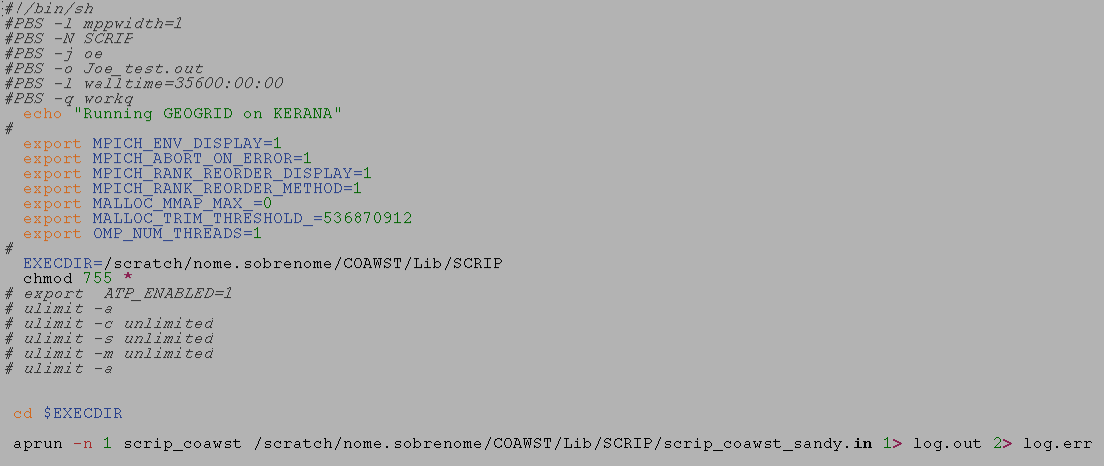
\includegraphics[width=0.65\textwidth]{scripqsub.png}
    \caption{Arquivo \textit{.sh} usado para executar o SCRIP.}
    \label{qsubscripsh}
\end{figure}
\bigskip

\noindent Para iniciar o SCRIP, digite:
\bigskip

\begin{bashcode}
qsub qsub_scrip.sh
\end{bashcode}
\bigskip

\noindent Ao final será criado o arquivo \textit{scrip\_static.nc}. Agora coloque-os na pasta do seu projeto e pronto! O COAWST está pronto para ser executado.
\bigskip

\section{Executanto seu projeto no COAWST}
\bigskip

\noindent Agora, com suas condições e grades prontas, seu projeto está pronto para ser executado. Visite a Seção \textcolor{bleu_cite}{\ref{sandyexec}} para relembrar como executar o projeto.
